%Correct the file name.
%X: book number
%Y: part number
%ZZZ: page number in three digits. So page 3 would be 003.

\documentclass[11pt]{amsbook}

\usepackage{../HBSuerDemir}	% ------------------------


\begin{document}

% ++++++++++++++++++++++++++++++++++++++
\hPage{b2p1/143}
% ++++++++++++++++++++++++++++++++++++++
	is a Vector Space $ M_{mxn} ( + , \mathbb{R} )$ where the inner product (dot product) is defined as \\
	\begin{center}
		$<A,B> = A.B = a_{11}b_{11} + ... + a_{1n}b_{1n} $ \\
		\quad \quad \quad \quad \quad \quad \text{  } $+ a_{21}b_{21} + ... + a_{2n}b_{2n}$ \\
		\quad \quad \quad \quad \quad \quad \quad$+a_{n1}b_{n1} + ... + a_{nn}b_{nn}$ \\
	\end{center}

	and the norm of A, by $ \hAbs{\hAbs{A}} = \sqrt{A.A}  $
	\begin{center}		
		The vector space $ R^3(+, \mathbb{R})$ has the natural generalization \\
		$R^{n}(+, . , R)$ \\
	\end{center}
	where
	\begin{center}
		$ R^n = \{ (x_{1}, ... , x_{n}): x_{i} \in R \} $ \\
	\end{center}
	is the set of all ordered n-tuples or vectors in n-space,in which 
	the operation of addition, multiplication by scalars and inner
	product are defined as: 
	\begin{center}
		$(x_{1}, ... , x_{n}) + (y_{1}, ... , y_{n}) = (x_{1}+y_{1}, ... , x_{n}+y_{n}) $ \\
		\quad \text{ } $ \lambda(x_{1}, ... , x_{n}) = (\lambda x_{1}, ... , \lambda x_{n})$ \\
		$(x_{1}, ... , x_{n}). (y_{1}, ... , y_{n}) = x_{1}y_{1} + ... + x_{n}y_{n} $ \\
	\end{center}
	\quad The vectors \\
	\quad $ e_{1} = ( 1, 0, ... , 0) ,  e_{2} = (0, 1, 0, ... 0), ... ,  e_{n}=(0, ... , 0,1) $ \\
	is this space are unit vectors and pairwise orthogonal as seen by \\
	application inner product:
	\begin{center}
		$ e_{i}.e_{j}  = $
		$\begin{cases}
			1 \text{ } when \text{ } i=j \\
			0\text{ } when \text{ } i \neq j 
		\end {cases} $

	\end{center}
	They are said to lie on $n (>1)$ mutually orthgonal axes $0_{x_{1}}, ... , 0_{x_{n}}$ \\
	sketch of which cannot be realized when $n>3.$

			







% =======================================
%\section{aaaah}






% =======================================
%\subsection{bbb}





% =======================================
%\subsubsection{cccc}

%This is the first figure. 
%\begin{figure}[htb]
%	\centering
%	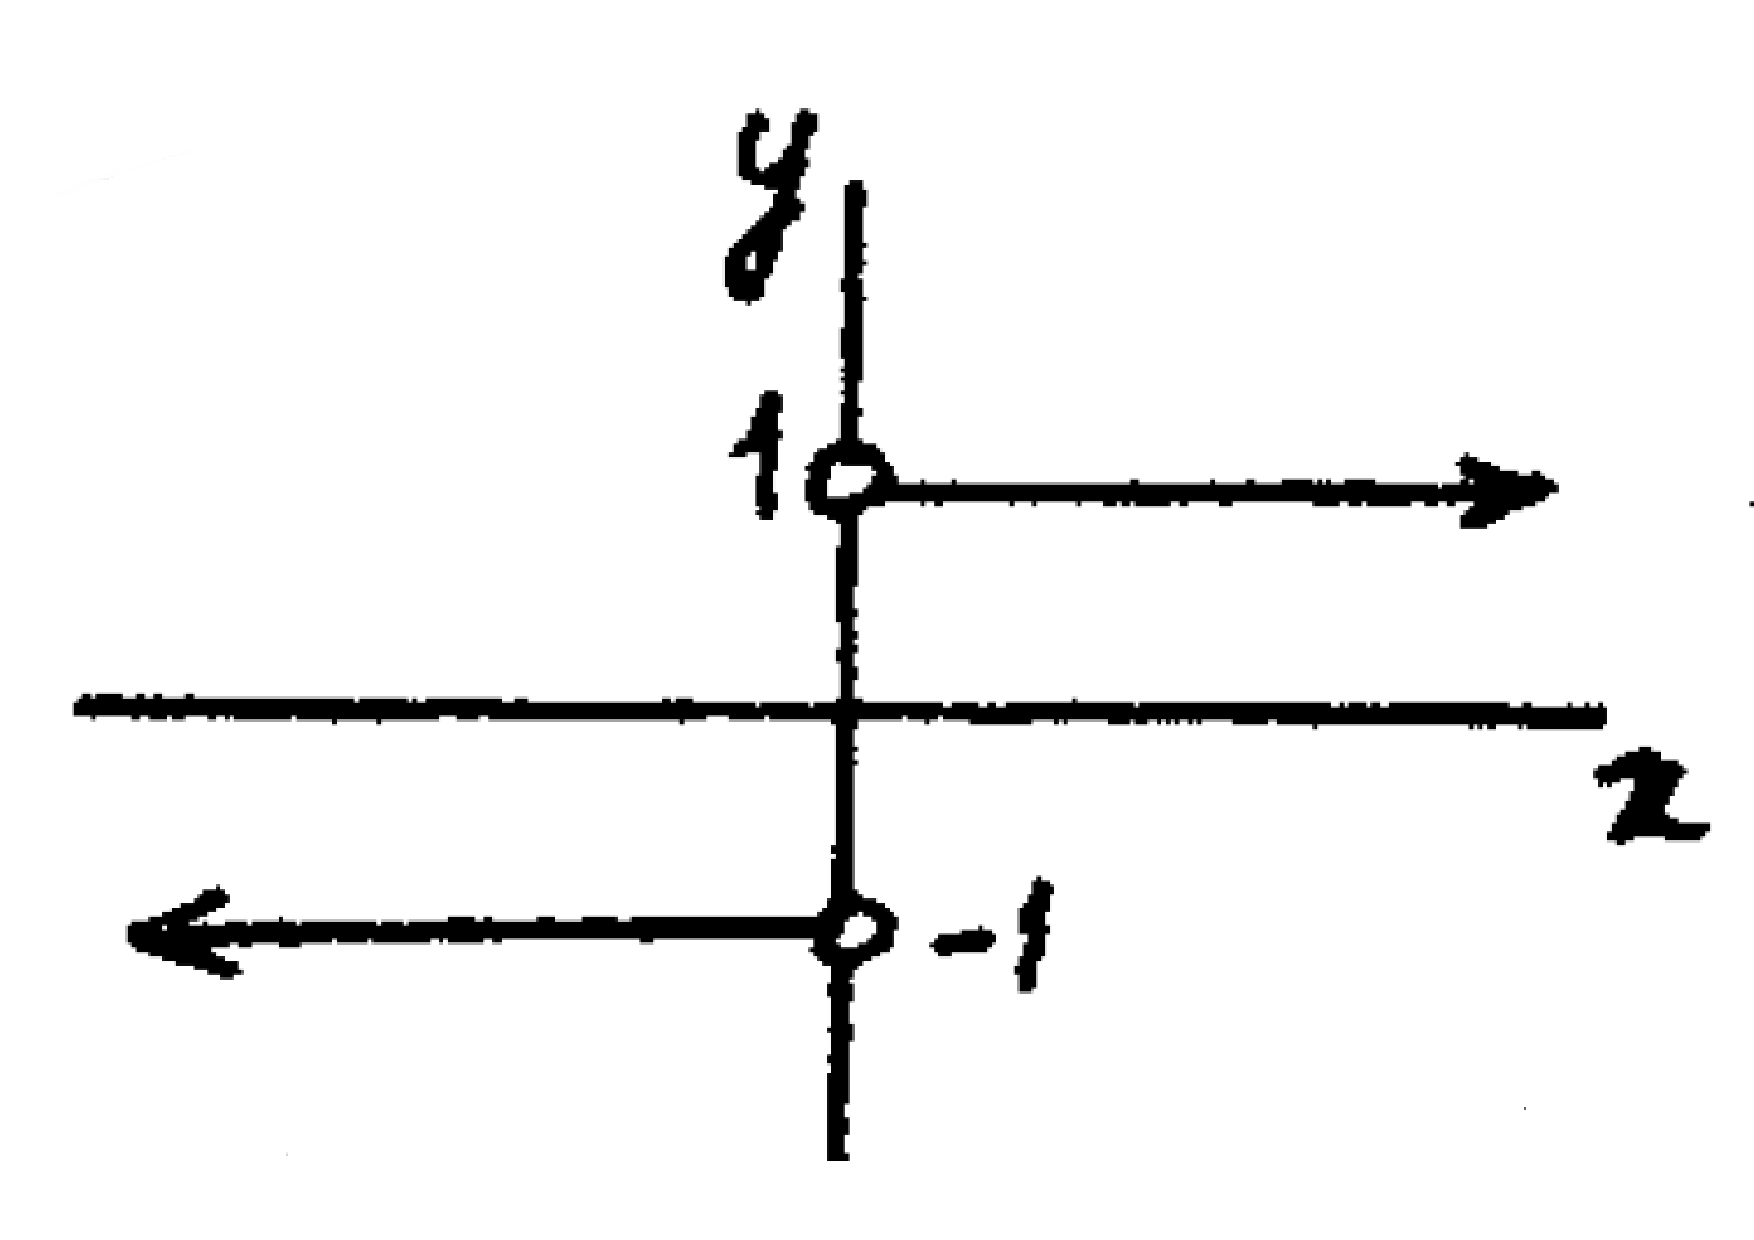
\includegraphics[width=0.45\textwidth]{images/bXpY-ZZZ-fig01}
%	\caption{Classification of complex numbers}
%	\label{fig:classificationOfComplexNumbersA}
%\end{figure}
%This is the second figure
%\begin{figure}[htb]
%	\centering
%	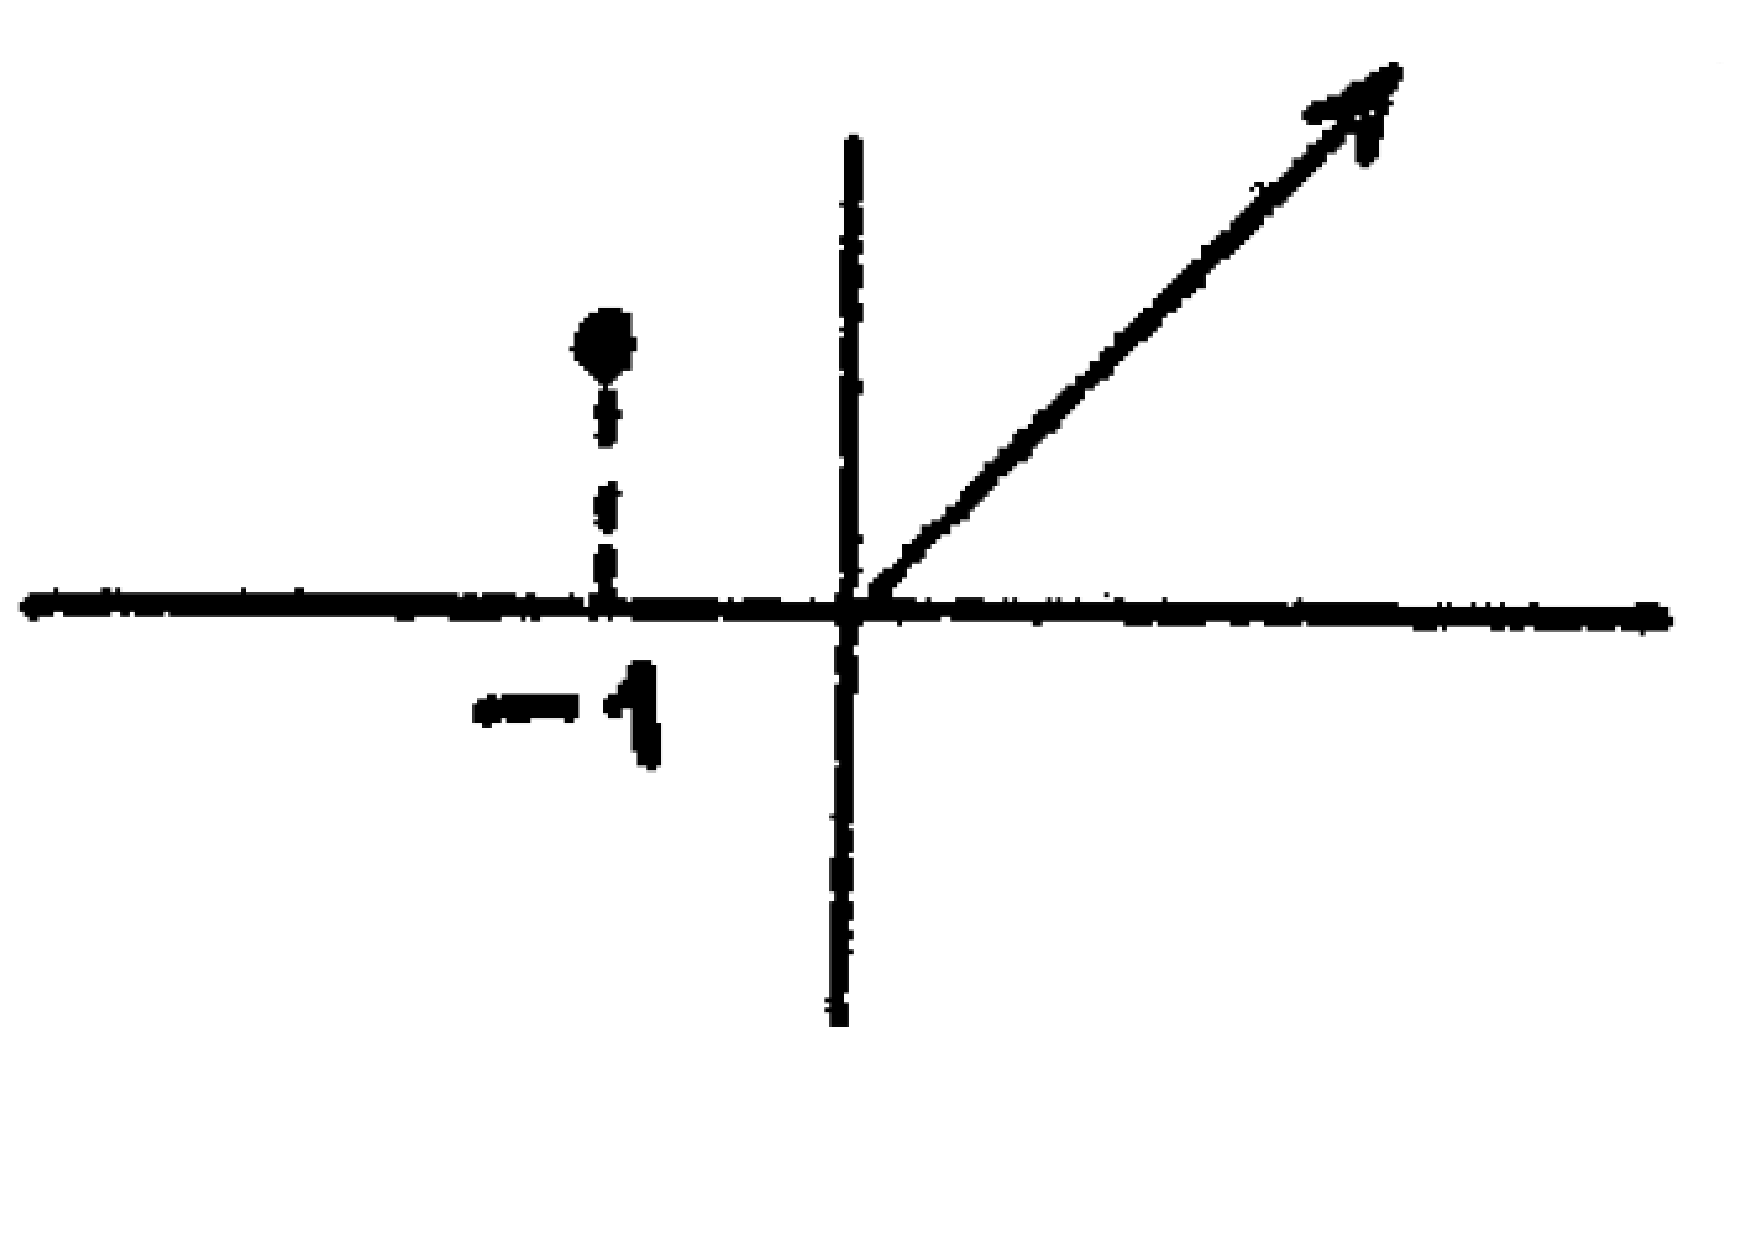
\includegraphics[width=0.45\textwidth]{images/bXpY-ZZZ-fig02}
%	\caption{Classification of complex numbers}
%	\label{fig:classificationOfComplexNumbersA}
%\end{figure}






% =======================================================
\end{document}  

%==== templates ====

%==== environments ====

%\begin{figure}[htb]
%	\centering
%	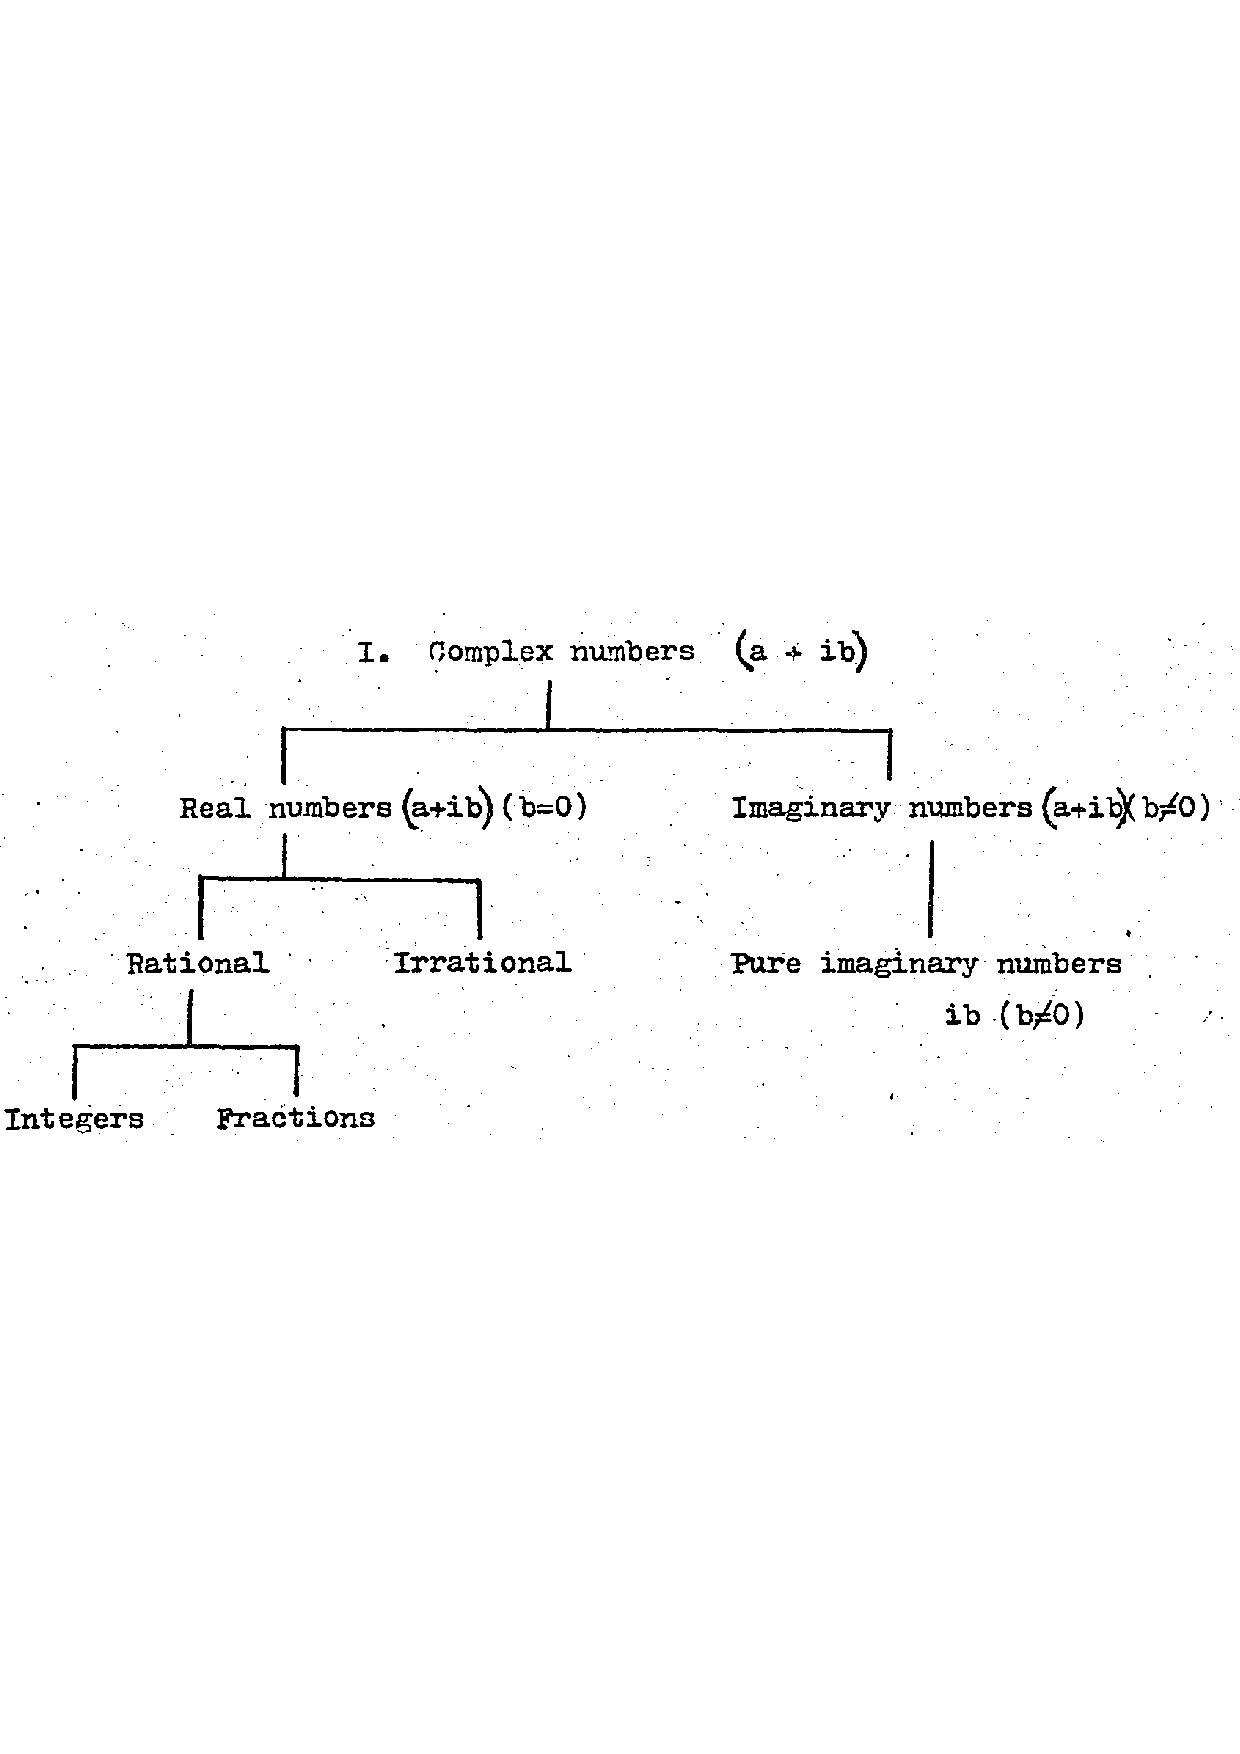
\includegraphics[width=0.9\textwidth]{images/SD-1-1p15A}
%	\caption{Classification of complex numbers}
%	\label{fig:classificationOfComplexNumbersA}
%\end{figure}

%\begin{center}
%\begin{tabular}{cc}
%\end{tabular}
%\end{center}

%\begin{exmp}
%\begin{hSolution}
%\end{hSolution}
%\end{exmp}

%\begin{hEnumerateAlpha}
%\end{hEnumerateAlpha}

%\begin{hEnumerateRoman}
%\end{hEnumerateRoman}

%$
%\begin{bmatrix}
%\end{bmatrix}
%$

%\frac{aaaa}{bbb}
%\frac{a_{n}}{b_{n}}
%\left( aaaa \right)
%\Longrightarrow

%\begin{multicols}{2}
%	bb
%\columnbreak
%	aa
%\end{multicols}
